% 2009 年四川卷文科第 6 题：正六棱锥 P-ABCDEF，PA⊥底面，PA=2AB。
% 来源 PDF：普通高考/2009/2009四川文.pdf，SHA256 2bb14d3824466d9566238b20ec9270686c67d6e4f2af4186fd22b2a14e633ea7
% 原页：第 1 页（A3 三栏）第 1 栏下部，印刷页 559。
% 重绘依据：底面正六边形 A 在左前、B 在右前、C 右后、D 后、E 左后、F 左；P 在 A 正上方；
%   可见棱 PA、PB、PC、PD 实线，PE、PF 与底面后侧两边虚线；标注按顶点外法向避让。
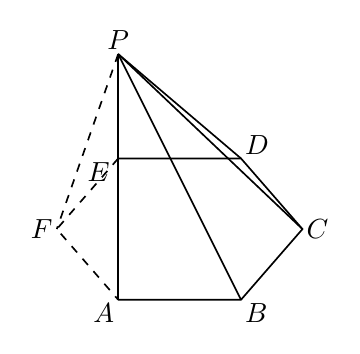
\begin{tikzpicture}[scale=0.78, semithick, every node/.style={inner sep=1.2pt}]
  \coordinate (A) at (0,0);
  \coordinate (B) at (2,0);
  \coordinate (C) at (3,1.15);
  \coordinate (D) at (2,2.3);
  \coordinate (E) at (0,2.3);
  \coordinate (F) at (-1,1.15);
  \coordinate (P) at (0,4.0);
  \draw[dashed] (E) -- (F) -- (A);
  \draw (A) -- (B) -- (C) -- (D) -- (E);
  \draw (P) -- (A);
  \draw (P) -- (B);
  \draw (P) -- (C);
  \draw (P) -- (D);
  \draw[dashed] (P) -- (E);
  \draw[dashed] (P) -- (F);
  \node[anchor=south] at (P) {$P$};
  \node[anchor=north east] at (A) {$A$};
  \node[anchor=north west] at (B) {$B$};
  \node[anchor=west] at (C) {$C$};
  \node[anchor=south west] at (D) {$D$};
  \node[anchor=north east] at ([xshift=-2pt]E) {$E$};
  \node[anchor=east] at (F) {$F$};
\end{tikzpicture}
